
\documentclass[10pt,twocolumn,letterpaper]{article}

\usepackage{iccv}
\usepackage{times}
\usepackage{epsfig}
\usepackage{graphicx}
\usepackage{amsmath}
\usepackage{amssymb}
\usepackage[numbers,sort]{natbib}
\usepackage[UTF8]{ctex}


\usepackage{subfigure}
\usepackage{upgreek}
\usepackage{multirow}
\usepackage{color}
\usepackage{bm}
\DeclareMathOperator*{\argmin}{arg\,min}
\usepackage{arydshln}
\usepackage{latexsym}

\usepackage{amsthm}
\newtheorem{theorem}{Theorem}
\newtheorem{lemma}[theorem]{Lemma}
\newtheorem{conj}[theorem]{Conjecture}

% Include other packages here, before hyperref.

% If you comment hyperref and then uncomment it, you should delete
% egpaper.aux before re-running latex.  (Or just hit 'q' on the first latex
% run, let it finish, and you should be clear).
\usepackage[pagebackref=true,breaklinks=true,letterpaper=true,colorlinks,bookmarks=false]{hyperref}

% \iccvfinalcopy % *** Uncomment this line for the final submission

\def\iccvPaperID{1} % *** Enter the ICCV Paper ID here
\def\httilde{\mbox{\tt\raisebox{-.5ex}{\symbol{126}}}}

% Pages are numbered in submission mode, and unnumbered in camera-ready
\ificcvfinal\pagestyle{empty}\fi
\begin{document}

%%%%%%%%% TITLE
\title{A Benchmark Dataset for Evaluating Denoising and Demosaicking Algorithms}

\author{First Author\\
Institution1\\
Institution1 address\\
{\tt\small firstauthor@i1.org}
% For a paper whose authors are all at the same institution,
% omit the following lines up until the closing ``}''.
% Additional authors and addresses can be added with ``\and'',
% just like the second author.
% To save space, use either the email address or home page, not both
\and
Second Author\\
Institution2\\
First line of institution2 address\\
{\tt\small secondauthor@i2.org}
}

\maketitle
%\thispagestyle{empty}


%%%%%%%%% ABSTRACT
\begin{abstract}
这份报告介绍我们在科研中遇到的三个问题,以及我们提出的解决这三个问题的方案。第一个问题关于真实噪声图数据库的构建,我们提出同时利用空间和时间的信息去构建一个带有干净图的,且能同时用于real demosaicking和real image denoising的数据库,这个数据库建立在raw data上;第二个问题关于很多learning-based super-resolution, domain transfer的算法中关于mapping matrix的设计 ($\min_{\bm{W}}\|\bm{A}_{1}-\bm{W}\bm{A}_{2}\|$),在很多算法里,这个mapping matrix是不可逆的,我们提出一系列完全可逆且几何意义明确的mapping matrices,可用于设计example-based super-resolution,domain transfer learning里的算法;第三个问题是稀疏表达框架下的正交字典学习模型和双边正交字典学习模型的收敛性问题,和加速问题。我们要用尽可能简单的方法证明正交字典学习模型和双边正交字典学习模型的收敛性,并采用Cayley transform设计新算法,从而提升带有正交约束($\bm{X}^{\top}\bm{X}=\bm{I}$)或正规化约束($\|\bm{x}\|_{2}=1$)的大量优化算法(如字典学习)的速度。
\end{abstract}

%%%%%%%%% BODY TEXT
\section{问题1:真实噪声图数据库的构造}

Nam et al.在发表于CVPR2016的文章\cite{crosschannel2016}里构造了一个带有``ground truth''的真实噪声图数据库,作者通过其连续拍摄500张RGB空间里的图片并且取平均来构造``ground truth'', 但是这个构造方法存在很多问题。

主要问题1:这些图片是在RGB空间上取平均的,这是不合理的。噪声只有在raw data上才满足每个像素独立的分布,且真实噪声只有在raw data上才符合泊松分布和高斯分布,光子进入传感器可以用泊松分布来拟合,所以这部分噪声是泊松分布的。由热量产生的Dark Current噪声是泊松分布的。在readout等阶段的噪声是符合高斯分布的。但是这些分布在digital camera pipeline里经过复杂的操作,这些噪声已经不再独立,也不再是泊松分布和高斯分布的了。

主要问题2:连续拍摄500张图持续时间必然很长,对周围环境要求过高。因此这个方法只能用于拍摄固定光源下的,室内的,静态的物体。无法拍摄人像,自然光下的物体,在短时间内静止但是在长时间内可能有轻微运动的物体。举个例子,Nikon A7II相机1秒钟只能连续拍摄60张图片,拍摄500张图片需要9分钟左右,即便是在室内,如果有自然光招进来,那么自然光的变化会严重影响拍摄的光照条件。在室外拍摄的时候,连续拍摄9分钟更加不可能拍摄到内容和光照一致的连续500张图片。

主要问题3:连续拍摄500张图像,raw data的像素有很大可能存在位移(shift),从而导致Color Filter Array (CFA)图片的R, G, B通道上的数值产生位移,从而导致demosaicking的时候产生偏差。 另外,还会使得图片的edge部分产生zippering的瑕疵、texture部分产生轻微模糊等问题。

主要问题4:连续拍摄500张会使得相机的传感器因为连续工作产生大量的热,从而使得相机在后续拍摄中产生大量的电子,温度越高,噪声越大,就是如下相机噪声模型中的$\bm{D}$的均值和方差越大。
\begin{equation}
\bm{P} = f((g_{cv}(\bm{C}+\bm{D})+\bm{N}_{reset})g_{out}+\bm{N}_{out})+\bm{Q}
\end{equation}

主要问题5:连续拍摄500张图取平均,那么传感器的每个pixel产生的噪声还带有该pixel本身的属性,这个由于物理性质本身产生的噪声无论如何也无法通过平均去掉,比如某个pixel总是把测量到的数值变大,这个测量值与真实值之间的差异无法通过自身上的平均消除。如果再借用空间上的信息,那么这个pixel产生的总是偏大噪声可以被周围pixel的测量值拉回到平均位置。


主要问题6:对于某些特定的相机,比如DJI的无人机Phonton 3,其只能一次性连续拍摄10张左右的照片。在下一次连续拍摄的时候,相机会自动进行聚焦等操作,而我们无法保证这些相机在相邻两次连续拍摄之间拥有完全一样的参数。只能把这一次性拍得的10张图片视为参数一致的图片数据,与之后连续拍摄的图片之间取平均会使得图片产生非常明显的位移和模糊。


解决办法:对于问题1,我们应该在raw data上取平均,而不是在RGB空间里取平均。对于问题2,3,4,5,我们可以用每张图片的空间信息来换取时间上的信息。我们不需要连续拍摄500张图片,也许只需要拍摄10张左右的图片,再利用空间上的信息就可以得到``ground truth''的图片了。如何利用空间上的信息呢?那就是在CFA上的RGGB像素里取平均,这个想法来自于微软公司的研究人员在CFA上做demosaicking数据库的构造\cite{khashabi2014joint}。这也是我们接下来要介绍的只在CFA空间域里取平均构建``ground truth''的工作。


Khashabi et al.在发表于TIP2014的文章\cite{khashabi2014joint}里构造了一个数据量很大的demosaicking的数据库,作者对于每个场景都做下采样。在下采样的过程中,把大小为$W\times W$的块中的代表某个颜色(比如红色)的所有像素取平均,然后下采样成一个像素;在右侧相邻的$W\times W$块中对另一个颜色(比如绿色)的所有像素取平均,然后下采样成一个像素;在下方响铃的$W\times W$块中对一个颜色(比如绿色)的所有像素取平均,然后下采样成一个像素;在右下方响铃的$W\times W$块中对另一个颜色(比如蓝色)的所有像素取平均,然后下采样成一个像素。这样就可以把一个$2W\times2W$的CFA中的块下采样成一个大小为$2\times2$的块,而且是符合``RGGB''的采样pattern(对其他采样pattern也可以用类似的方法)。这个下采样模式可以通过图1表示。

\begin{figure}
\centering
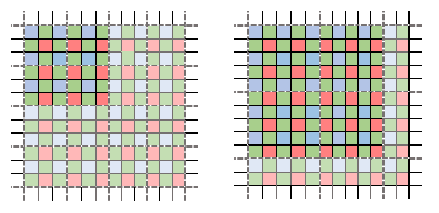
\includegraphics[width=0.95\linewidth]{CFA.png}
\caption{Averaging with odd windows, with $W = 1$ (left) and $W = 2$ (right),
where the window size is $(2W + 1)\times (2W + 1)$.
}
\label{fig1}
\end{figure}


主要问题1:存在图片像素过小,每张图片只有$200\times200$的大小。这是因为,为了得到干净的CFA图片,需要采用很大的下采样倍数。比如原图可能有$4000\times4000$,但是为了得到干净的CFA图片,采用$20\times20=400$倍的下采样倍数,才能得到一张非常干净的CFA图片可以用于做真实的demosaicking实验。这极大地降低了图片的内容和多样性,失去了图片原有的文理信息。这种失真严重的结果就是,在这个数据集上训练得到的demosaicking的算法不鲁棒,很容易遇到这个训练集上没有的图像块结构和文理信息。这时候我们可以借用时间上的信息,比如同样的图片拍摄10张,这10张的拍摄在0.1秒左右,在可控制的情况下,图片内容是可以保持不变的。在这种情况下,也许在空间上,我们不需要下采样那么多倍数,可以只下采样$4\times4=16$倍左右,那么依然可以得到$1000\times1000$大小的图片,依然可以保留大部分的文理,同时还可以得到质量一样的``ground truth''。

综上所述,我们可以结合时间上的多次采样和空间上的下采样,得到可以同时用于真实去噪和真实demosaicking的数据库。这个数据库还有用于真实的超分辨算法训练的潜在的可能性。

\section{问题2:基于学习的超分辨算法,迁移学习算法中的映射矩阵问题}
我们用超分辨算法举例,在example-based的超分辨算法里,有一步很关键,那就是高分辨图和低分辨图之间的映射矩阵。假设是基于字典学习做超分辨,在低分辨率图像块的字典上的系数是$\bm{A}_{1}$, 在高分辨率图像块的字典上的系数是$\bm{A}_{2}$,那么需要有一个映射矩阵$\bm{W}$使得$\bm{A}_{1}$尽可能接近$\bm{W}\bm{A}_{2}$。这本质上就是一个逼近的问题,可以在orthogonal Procrustes的框架里找到非常丰富的理论和应用。但是之前所有的方法中$\bm{W}$是无法保证可逆的,而且设计原则是非常不合理的。



在这里我们主要提出如下的解决方案
\begin{equation}
\min_{\bm{W}}\|\bm{A}_{1}-(\bm{W}\bm{A}_{2}+\bm{B})\|_{F}^{2}
\quad
\text{s.t.}
\quad
\bm{W}^{\top}\bm{W}=\bm{I}.
\end{equation}
其中$\bm{W}$负责旋转变换,$\bm{B}$负责平移变换。把这个框架嵌入到目前已有的算法中(比如SCDL),然后用这个模型用于真实图像去噪(在上述创建的数据库上训练),demosaicking,和超分辨,迁移学习等应用上。

我们也可以提出isotropic orthogonal procrustes analysis,这是一个各向同性的线性变换:
\begin{equation}
\min_{\bm{W}, \alpha, \bm{B}}\|\bm{A}_{1}-(\alpha\bm{W}\bm{A}_{2}+\bm{B})\|_{F}^{2}
\quad
\text{s.t.}
\quad
\bm{W}^{\top}\bm{W}=\bm{I},
\end{equation}
其中$\bm{W}$是正交旋转矩阵;$\alpha$是scale factor,用于伸缩旋转矩阵; $\bm{B}$是每列都相同的矩阵,用于平移变换。这里的$\bm{W}, \alpha, \bm{B}$都有闭合解。

我们还可以提出anisotropic orthogonal procrustes analysis,这是一个各向异性的非线性变换:
\begin{equation}
\min_{\bm{W}, \bm{S}}\|\bm{A}_{1}-(\bm{S}\bm{W}\bm{A}_{2}+\bm{B})\|_{F}^{2}
\quad
\text{s.t.}
\quad
\bm{W}^{\top}\bm{W}=\bm{I},
\end{equation}
这里$\bm{S}$是一个对角矩阵。同样地,$\bm{W},\bm{S},\bm{B}$都有闭合解,$\bm{S}$的闭合解还有待确认。




\section{问题3:对正交字典学习和双边正交字典学习模型进行加速}

\subsection{对正交字典学习模型进行加速}
稀疏表达下的正交字典学习模型如下:
\begin{equation}\label{equ5}
\min_{\bm{D},\bm{C}}\|\bm{Y}-\bm{D}\bm{C}\|_{F}^{2}
+
\lambda\|\bm{C}\|_{1}
\quad
\text{s.t.}
\quad
\bm{D}^{\top}\bm{D} =\bm{I}. 
\end{equation}

a. update $\bm{C}$
\begin{equation}
\min_{\bm{C}}\|\bm{D}^{\top}\bm{Y}-\bm{C}\|_{F}^{2}
+
\lambda\|\bm{C}\|_{1}.
\end{equation}
有闭合解。

b. update $\bm{D}$
\begin{equation}
\min_{\bm{D}}\|\bm{Y}-\bm{D}\bm{C}\|_{F}^{2}
\quad
\text{s.t.}
\quad
\bm{D}^{\top}\bm{D} =\bm{I}. 
\end{equation}
闭合解为:$\hat{\bm{D}}=\bm{V}\bm{U}^{\top}$, 其中$\bm{C}\bm{Y}^{\top}=\bm{U}\bm{\Sigma}\bm{V}^{\top}$是SVD分解。


Since the objective function of (\ref{equ5}) is monotonically non-increasing and has the lower bound (0), it is convergent according to the famous Monotone Convergence Theorem \cite{stein2009real}. It could be reasonably terminated when the decreasing rate is smaller than a preset threshold or the number of alternating updating steps of the optimization problem reaches the maximum iteration number. 

\subsection{对双边正交字典学习模型进行加速}

稀疏表达下的双边(two-sided)正交字典学习模型如下:
\begin{equation}\label{equ5}
\min_{\bm{T},\bm{S},\bm{C}}\|\bm{Y}-\bm{T}\bm{C}\bm{S}\|_{F}^{2}
+
\lambda\|\bm{C}\|_{1}
\quad
\text{s.t.}
\quad
\bm{T}^{\top}\bm{T} =\bm{I},
\bm{S}^{\top}\bm{S} =\bm{I}. 
\end{equation}


a. update $\bm{C}$
\begin{equation}
\min_{\bm{C}}\|\bm{T}^{\top}\bm{Y}\bm{S}^{\top}-\bm{C}\|_{F}^{2}
+
\lambda\|\bm{C}\|_{1}.
\end{equation}
有闭合解。

b. update $\bm{T}$ and $\bm{S}$
\begin{equation}\label{equ5}
\min_{\bm{T},\bm{S}}\|\bm{Y}-\bm{T}\bm{C}\bm{S}\|_{F}^{2}
\quad
\text{s.t.}
\quad
\bm{T}^{\top}\bm{T} =\bm{I},
\bm{S}^{\top}\bm{S} =\bm{I}. 
\end{equation}
闭合解为:$\hat{\bm{T}}=\bm{U}_{1}\bm{U}_{2}^{\top}$, $\hat{\bm{S}}=\bm{V}_{2}\bm{V}_{1}^{\top}$,
其中,$\bm{Y}^{\top}=\bm{U}_{1}\bm{\Sigma}_{1}\bm{V}_{1}^{\top}$,
$\bm{C}^{\top}=\bm{U}_{2}\bm{\Sigma}_{2}\bm{V}_{2}^{\top}$是SVD分解。

实验证实这两个模型都是收敛的。
目前为止,我没有看到有人证明这个模型的收敛性。
新加坡国立大学的Hui Ji的学生Chenglong Bao在论文\cite{bao2014convergent,bao2014l0,bao2016dictionary}证明了正交字典学习模型的一个退化模型的收敛性。但是其证明非常复杂,而且对理解这个模型没有太大帮助。



我们可以证明正交字典学习模型双边正交字典学习模型的收敛性。
此外,这两个模型每一次迭代里都有SVD分解,计算量非常大,我们可以参考论文\cite{wen2013feasible}的方法,运用Cayley Transform对这两个模型进行加速。同时运用论文中的\cite{edelman1998geometry}的方法,来研究双边字典学习模型的几何性质。这个Cayley Transform技术还可以用于对带有正规化向量约束的优化问题的提速。争取也能发在和论文\cite{bao2014convergent,bao2014l0,bao2016dictionary}同等水平的会议和期刊上。这两个模型可以用在图像修复上,比如去噪。只需要和K-SVD等一些传统字典学习的方法比较效果。





{
\small
\bibliographystyle{unsrt}
\bibliography{egbib}
}

\end{document}
